\documentclass[10pt,twocolumn]{article}
\usepackage[margin=1in]{geometry}
\usepackage{amsmath, amssymb}
\usepackage{graphicx}
\usepackage{hyperref}
\usepackage{setspace}
\usepackage{caption}
\usepackage{subcaption}
\usepackage{booktabs}

% Project title.
\title{Optimization of Regularized Matrix Factorization for Movie Recommendation Systems}

% Project "Dudes".
\author{Iliana Platona\\(csdp1436)\and Charalampos Apostolou\\(csdp1415)}

% Date of Creation.
\date{\today}

\begin{document}
% Add title (+date, +authors) to project report.
\maketitle

% Section: "Abstract".
\begin{abstract}
Recommender systems rely on predicting missing entries in highly sparse rating matrices. 
In this project, we formulate recommendation as a regularized matrix completion problem and study optimization methods for learning low rank latent factor models. 
We implemented Regularized Matrix Factorization (RMF), optimized it using Stochastic Gradient Descent (SGD) and evaluated its performance on the . 
Experimental results demonstrate that matrix factorization significantly outperforms baseline predictors. 
% while illustrating the classical bias--variance trade-off as the latent dimension increases. /* We'll see if this makes it */ 
\end{abstract}

% Section: "Introduction".
\section{Introduction}
Recommender systems are fundamental components of modern digital platforms. 
Their objective is to predict user preferences for items using partially observed interaction data.\\
The user item rating matrix is typically:
\begin{itemize}
    \item large,
    \item extremely sparse,
    \item noisy.
\end{itemize}
We address the recommendation problem as a \textbf{matrix completion} task using low rank approximation techniques. 
From an optimization perspective, this leads to a regularized non-convex minimization problem.

% Section: "Problem Formulation".
\section{Problem Formulation}
Let $R \in \mathbb{R}^{m \times n}$ denote the rating matrix and $\Omega$ the set of observed entries.\\
We approximate $R$ using a low-rank factorization:
\begin{equation}                    % Used "\begin{equation} to get "(1)" after equation.
R_{ij} \approx u_i^\top v_j
\end{equation}
\\
\\where:                            % New line here to move "where" to next column and make it prettier.
\begin{itemize}
    \item $u_i \in \mathbb{R}^K$ is the latent vector for user $i$,
    \item $v_j \in \mathbb{R}^K$ is the latent vector for item $j$,
    \item $K$ is the latent dimension.
\end{itemize}

% subsection: "Regularized Objective".
\subsection{Regularized Objective}
We solve:
\begin{equation}
\min_{U,V}
\sum_{(i,j)\in\Omega}
\left( R_{ij} - u_i^\top v_j \right)^2
+
\lambda \left( \|u_i\|^2 + \|v_j\|^2 \right)
\end{equation}
The objective is non convex jointly in $(U,V)$ but convex in each when the other is fixed.

% subsection: "Bias Augmented Model".
\subsection{Bias-Augmented Model}
To improve prediction quality, we include bias terms:
\begin{equation}
\hat{R}_{ij} = \mu + b_i + c_j + u_i^\top v_j
\end{equation}
where:                            % New line here to move "where" to next column and make it prettier.
\begin{itemize}
    \item $\mu$ is the global mean,
    \item $b_i$ is the $i_{th}$ user bias,
    \item $c_j$ is the $j_{th}$item bias.
\end{itemize}

% Section: "Optimization Method".
\section{Optimization Method}
We optimize the objective using \textbf{Stochastic Gradient Descent (SGD)}.
For each observed rating $(i,j)$, define the error:
\begin{equation}
e_{ij} = R_{ij} - \hat{R}_{ij}
\end{equation}
The updates are:
\begin{align}
u_i &\leftarrow u_i + \alpha ( e_{ij} v_j - \lambda u_i )\\
v_j &\leftarrow v_j + \alpha ( e_{ij} u_i - \lambda v_j )\\
b_i &\leftarrow b_i + \alpha ( e_{ij} - \lambda b_i )\\
c_j &\leftarrow c_j + \alpha ( e_{ij} - \lambda c_j )
\end{align}
where $\alpha$ is the learning rate.

% Section: "Dataset \& Experimental Setup".
\section{Dataset \& Experimental Setup}

% subsection: "Dataset".
\subsection{Dataset}
We use the \href{https://grouplens.org/datasets/movielens/latest/}{\textbf{Small "MovieLens" Dataset}}:
\begin{itemize}
    \item $\sim$ 100K ratings
    \item $\sim$ 600 users
    \item $\sim$ 9,000 movies
\end{itemize}

% subsection: "Evaluation Metric".
\subsection{Evaluation Metric}
Performance is evaluated using Root Mean Square Error (RMSE):
\begin{equation}
\text{RMSE} =\sqrt{\frac{1}{|\Omega_{test}|}\sum_{(i,j)\in\Omega_{test}}(R_{ij} - \hat{R}_{ij})^2}
\end{equation}

% Section: "Results".
\section{Results}

% subsection: "Convergence Analysis".
\subsection{Convergence Analysis}
SGD shows steady convergence across all tested latent dimensions. 
Training error decreases monotonically, confirming correct gradient implementation.

% Figure "convergence_plot.png".
\begin{figure}[ht]
    \centering
    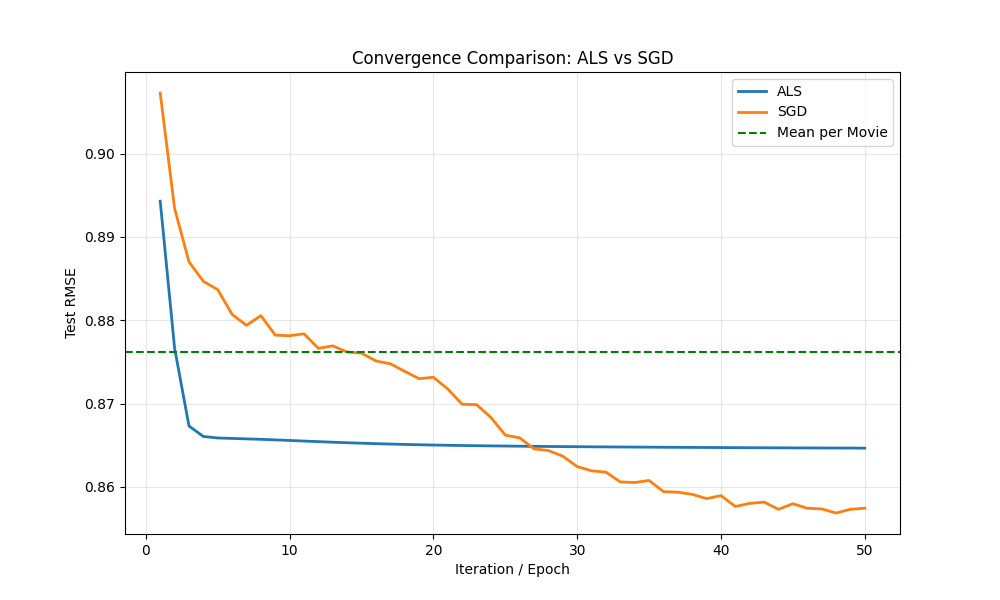
\includegraphics[width=0.45\textwidth]{figures/convergence_plot.png}
    \caption{Training RMSE as a function of epochs for different latent dimensions $K$.}
    \label{fig:training_curve}
\end{figure}

% subsection: "Effect of Latent Dimension".
\subsection{Effect of Latent Dimension}
Increasing $K$ improves training accuracy but may degrade generalization performance due to overfitting.

% ----------- INSERT GENERALIZATION GAP PLOT -----------
% \begin{figure}[h]
%     \centering
%     \includegraphics[width=0.45\textwidth]{figures/generalization_gap.png}
%     \caption{Training and test RMSE versus latent dimension $K$, illustrating the bias--variance trade-off.}
%     \label{fig:generalization}
% \end{figure}

\subsection{Comparison with Baselines}
Matrix factorization significantly outperforms:
\begin{itemize}
    \item Global mean predictor
    \item Item-based mean predictor
\end{itemize}

% Figure: "matrixpicture_tex-2.pdf".
\begin{figure}[ht]
    \centering
    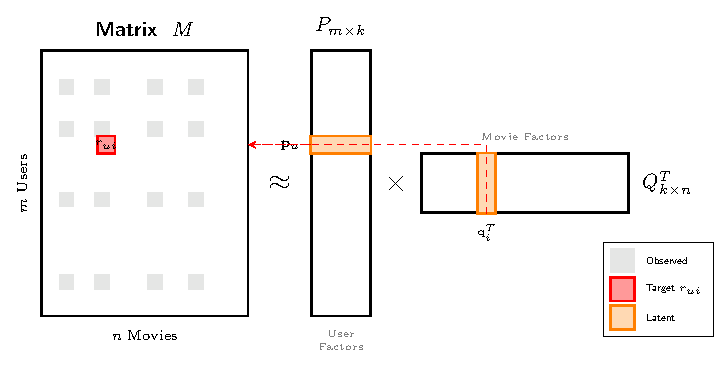
\includegraphics[width=0.45\textwidth]{figures/matrixpicture_tex-2.pdf}
    \caption{Comparison of RMSE between baseline predictors and matrix factorization.}
    \label{fig:baselines}
\end{figure}

% Section: "Discussion".
\section{Discussion}
From an optimization perspective:
\begin{itemize}
    \item The objective is non-convex but well-behaved in practice.
    \item SGD provides scalable optimization for sparse data.
    \item Regularization is essential to control overfitting.
    \item Increasing $K$ reveals the bias--variance trade-off.
\end{itemize}
Compared to Alternating Least Squares (ALS):
\begin{itemize}
    \item ALS solves convex subproblems exactly,
    \item SGD provides more flexibility and scalability.
\end{itemize}

% Section: "Conclusion".
\section{Conclusion}
We demonstrated that Regularized Matrix Factorization optimized via SGD effectively addresses sparse recommendation problems. 
The model substantially outperforms simple baselines and exhibits expected theoretical behavior with respect to model complexity and regularization.

% Section: "Future Work".
\section{Future Work}
Future directions include:
\begin{itemize}
    \item Implicit feedback modeling,
    \item Adaptive learning rate methods (Adam, RMSProp),
    \item Cross-validation for hyperparameter tuning,
    \item Hybrid recommendation models.
\end{itemize}

\end{document}